\documentclass[10pt,]{article}
\usepackage{lmodern}
\usepackage{amssymb,amsmath}
\usepackage{ifxetex,ifluatex}
\usepackage{fixltx2e} % provides \textsubscript
\ifnum 0\ifxetex 1\fi\ifluatex 1\fi=0 % if pdftex
  \usepackage[T1]{fontenc}
  \usepackage[utf8]{inputenc}
\else % if luatex or xelatex
  \ifxetex
    \usepackage{mathspec}
  \else
    \usepackage{fontspec}
  \fi
  \defaultfontfeatures{Ligatures=TeX,Scale=MatchLowercase}
\fi
% use upquote if available, for straight quotes in verbatim environments
\IfFileExists{upquote.sty}{\usepackage{upquote}}{}
% use microtype if available
\IfFileExists{microtype.sty}{%
\usepackage{microtype}
\UseMicrotypeSet[protrusion]{basicmath} % disable protrusion for tt fonts
}{}
\usepackage[margin=1.0in]{geometry}
\usepackage{hyperref}
\hypersetup{unicode=true,
            pdftitle={Department Invited Speakers Do Not Reflect Trainee Diversity},
            pdfborder={0 0 0},
            breaklinks=true}
\urlstyle{same}  % don't use monospace font for urls
\usepackage{graphicx,grffile}
\makeatletter
\def\maxwidth{\ifdim\Gin@nat@width>\linewidth\linewidth\else\Gin@nat@width\fi}
\def\maxheight{\ifdim\Gin@nat@height>\textheight\textheight\else\Gin@nat@height\fi}
\makeatother
% Scale images if necessary, so that they will not overflow the page
% margins by default, and it is still possible to overwrite the defaults
% using explicit options in \includegraphics[width, height, ...]{}
\setkeys{Gin}{width=\maxwidth,height=\maxheight,keepaspectratio}
\IfFileExists{parskip.sty}{%
\usepackage{parskip}
}{% else
\setlength{\parindent}{0pt}
\setlength{\parskip}{6pt plus 2pt minus 1pt}
}
\setlength{\emergencystretch}{3em}  % prevent overfull lines
\providecommand{\tightlist}{%
  \setlength{\itemsep}{0pt}\setlength{\parskip}{0pt}}
\setcounter{secnumdepth}{0}
% Redefines (sub)paragraphs to behave more like sections
\ifx\paragraph\undefined\else
\let\oldparagraph\paragraph
\renewcommand{\paragraph}[1]{\oldparagraph{#1}\mbox{}}
\fi
\ifx\subparagraph\undefined\else
\let\oldsubparagraph\subparagraph
\renewcommand{\subparagraph}[1]{\oldsubparagraph{#1}\mbox{}}
\fi

%%% Use protect on footnotes to avoid problems with footnotes in titles
\let\rmarkdownfootnote\footnote%
\def\footnote{\protect\rmarkdownfootnote}

%%% Change title format to be more compact
\usepackage{titling}

% Create subtitle command for use in maketitle
\newcommand{\subtitle}[1]{
  \posttitle{
    \begin{center}\large#1\end{center}
    }
}

\setlength{\droptitle}{-2em}

  \title{\textbf{Department Invited Speakers Do Not Reflect Trainee Diversity}}
    \pretitle{\vspace{\droptitle}\centering\huge}
  \posttitle{\par}
    \author{}
    \preauthor{}\postauthor{}
    \date{}
    \predate{}\postdate{}
  
\usepackage{booktabs}
\usepackage{longtable}
\usepackage{array}
\usepackage{multirow}
\usepackage[table]{xcolor}
\usepackage{wrapfig}
\usepackage{float}
\usepackage{colortbl}
\usepackage{pdflscape}
\usepackage{tabu}
\usepackage{threeparttable}
\usepackage{threeparttablex}
\usepackage[normalem]{ulem}
\usepackage{makecell}
\usepackage{caption}

\usepackage{helvet} % Helvetica font
\renewcommand*\familydefault{\sfdefault} % Use the sans serif version of the font
\usepackage[T1]{fontenc}

\usepackage[none]{hyphenat}

\usepackage{setspace}
\doublespacing
\setlength{\parskip}{1em}

\usepackage{lineno}

\usepackage{pdfpages}
\floatplacement{figure}{H} % Keep the figure up top of the page

\begin{document}
\maketitle

\vspace{30mm}

Running title: Invited Speaker Diversity Does Not Reflect Trainee
Diversity

\vspace{35mm}

Ada K. Hagan, Ph.D.\({^1}\)\^{}, Rebecca M. Pollet, Ph.D.\({^1}\)\^{},
and Josie Libertucci, Ph.D.\({^2}\)\^{}

\vspace{35mm}

\(\dagger\) To whom correspondence should be addressed:
\href{mailto:akhagan@umich.edu}{\nolinkurl{akhagan@umich.edu}} or
\href{mailto:libertj@mcmaster.ca}{\nolinkurl{libertj@mcmaster.ca}}

1. Department of Microbiology \& Immunology, University of Michigan, Ann
Arbor, Michigan

2. Department of Medicine, McMaster University, Hamilton, Ontario,
Canada

Figures:

Tables:

Supplemental:

\newpage

\linenumbers

\subsection{Abstract}\label{abstract}

\subsection{Keywords}\label{keywords}

inclusion, diversity, invited speakers, academia, graduate programs

\newpage

\subsection{Background}\label{background}

500 words

Representation of white women and historically underrepresented
minorities (HURM) in science, technology, engineering, and math (STEM)
in the workforce remains low despite equal enrollment in undergraduate
STEM majors. Longitudinal data indicates that these discrepancies might
be partially explained by low retention of women and URM in
undergraduate STEM programs where academic performance is a key
predictor of retention. A growing body of evidence suggests that women
and URM under-perform in introductory science courses compared to their
white male colleagues, even when representation is equal. Additionally,
there is evidence to suggest that women and URM participate less in
class, which could inhibit the learning process and subsequent success.
A prevailing hypothesis to explain achievement gaps and a lack of
participation in class for women and URM is that, many students have an
unconscious fear of being seen as a negative stereotype, termed
stereotype threat. This is prevalent in fields that have historically
been dominated by white males, such as in STEM. In order to retain a
diverse population of students in STEM, in an effort to ensure all
students have equal opportunities and resources to be successful,
under-performance and a lack of participation in introductory science
courses needs to be addressed. One mechanism to address the issue is
through the use of inclusive teaching practices --teaching methods that
promote the full participation, learning, and success of all students.

\begin{itemize}
\item
  introduce invited speaker series - what are the goals, who attends,
  etc.
\item
  previous examinations have focused on conferences and panels, large
  number of people in a short period of time -- easy to make comparisons
  \& see trends
\item
  more difficult to see trends over long time period -- asked cumulative
  trends of speakers over 5 year period, ``normative'' to trainees in
  the department
\end{itemize}

\subsection{Methods}\label{methods}

Each academic year, each faculty member in the Department of
Microbiology and Immunology at the University of Michigan has the
opportunity to invite one speaker per year for a weekly seminar series.
Some of these seminar slots are dedicated to named lectureships, which
are decided by committee, and three trainee-invited speakers. We
analyzed the gender and demographics of invited speakers and faculty
hosts for five academic years (Fall 2014 - Spring 2019), and the current
trainees when the data were analyzed (Spring 2019).

Each speaker was only counted once and any departmental faculty members
or those listed as a ``host'' at any point could not also be considered
``invited speakers''. The list of faculty hosts was used as a proxy for
faculty demographics since as hosts, these faculty members are visible
representatives of the department. The list of trainees was obtained
from department listservs and included masters students, doctoral
students, and post-doctoral fellows.

We hand-coded demographics using personal knowledge, photos, and CVs.
The presenting gender if each invidual was assigned using a binary
system (man/woman). Diversity definitions vary according to the goals
and population in question. However, in the United States, there is an
inclination to consider both individuals of historically
under-represented minority (HURM) and international backgrounds
together. We argue that it is important to distinguish these two groups
separately since each face different issues in the US and the academy
and thus require different support systems. For instance, international
scientists must contend with visa issues while HURMs have the trauma
associated with living in a country who systematically shuts them out
(despite an infrastructure that was built on their historical land and
labor). For this reason, other assigned demographics included Caucasian,
Historically Under-represented Minority (HURM), and International, each
with a binary (yes/no) possibilty. Caucasian was assigned using the
current U.S. Census definition where those of Middle Eastern, European,
and Russian descent are included. HURM individuals were restricted to
those with African-American, Indigenous and/or Hispanic heritage while
International individuals were either visiting the US at the time of
their talk, or immigrated to the US as an adult.

\subsection{Results and Discussion}\label{results-and-discussion}

To understand the representation of women, we compared the proportion of
individuals presenting as women in each academic role. At the trainee
level, more than half of students and postdoctoral fellows were women.
That dropped to X\% of faculty hosts and X\% of the invited speakers. 10
of 31 lectureships {[}what about lectureships?{]} The proportion of
women as faculty hosts and speakers is equivalent to global estimates of
women microbiologists (Elseiver). Several papers have investigated the
representation of women at scientific conferences, however, we only
identified one that focused on invited speakers at university-sponsored
events (Nittrouer, 2018). {[}Compare to our findings{]}

Assumptions about competency and dedication may negatively impact the
likelihood of women microbiologists being invited as speakers. The
dedication of women with family to their work is also more likely to be
questioned than that of their colleagues, even men who also have
children. For instance, the perceived prioritization and commitments of
women to family over work may cause faculty to doubt their acceptance of
a speaking invitation (despite the prestigious nature of these
invitations), causing the faculty member to invite a different colleague
who they feel is less likely to turn them down. Departments have
different processes and criteria for selecting invited speakers, but
want to bring the best scientists possible. It may be that the
definition of ``best'' poses a problem to women, who need three-times as
many publications as their men colleges to be considered equally
competent. Some departments only invite tenured faculty, which severely
limits the number of potential women speakers considerably. Alternately,
pre-tenure faculty members invite prestigious, tenured faculty in their
field to network and secure letters for their own tenure package. The
increased burden of women to prove competency decreases their likelihood
to be considered for either tenure and as possible source of tenure
letters.

Our analysis identified an over-representation of Caucasian individuals
as hosting faculty and invited speakers, relative to the proportion of
Caucasian trainees. We observed declines in the representation of HURM
and international faculty and speakers relative to the trainees.

{[}Lectureships{]}. 22, 3, 6, (cauc, HURM, Internatl, respectively) --
12, 10, 5, 0 (CaucM, CaucW, Non-CaucM, Non-CaucW)

\subsection{Call to Action}\label{call-to-action}

\begin{itemize}
\tightlist
\item
  Improving speaker diversity

  \begin{itemize}
  \tightlist
  \item
    US-serving institutions have particular responsibility to those
    historically suppressed populations
  \item
    to improve retention of white women \& HURMs, each group needs
    equivalent representation to counteract biases and improve
    self-efficacy
  \item
    recall bias not the only issue, also not always possible to identify
    members of historically under-served communities
  \item
    example: there are speakers who have URM status, but it wasn't
    readily apparent from the internet/CV
  \item
    perspective is often as/more important than self-identification
  \end{itemize}
\item
  Development of Diversify tools

  \begin{itemize}
  \tightlist
  \item
    inspired by EEB/Chemistry
  \item
    tool for members of URM groups to self-identify \& for others to use
    to find diverse candidates
  \item
    describe maintenance of lists (Rebecca)
  \item
    describe website creation
  \end{itemize}
\item
  Other resources/ideas

  \begin{itemize}
  \tightlist
  \item
    student/lab invited speakers -- improve diversity of suggestions
    (fields/careers)
  \item
    departments to invite speakers to share about their personal story
    as well as their science
  \end{itemize}
\end{itemize}

\subsection{Conclusion}\label{conclusion}

\begin{itemize}
\tightlist
\item
  increased retention of white women \& HURMS -- increasing
  representation of
\item
  tools available to create field specific lists of H under-served
\end{itemize}

\subsection{Acknowledgements}\label{acknowledgements}

We thank Harry Mobley and the Department of Microbiology \& Immunology,
University of Michigan for their support and input. We would also like
to acknowledge Nick Lesniak and Dr.~Ariangela Kozick for their comments
and suggestions.

\subsection{Author Contributions}\label{author-contributions}

A.K.H. collected the data, assigned demographics, analyzed the data, and
created the website. R.P. created the Google lists, forms, and website
content and the description of their maintenance. J.L. wrote the
introduction and provided conceptual advice. All authors contributed to
the final manuscript.

\subsection{Code and data
availability}\label{code-and-data-availability}

The anonymized data, code for all analysis steps, and an Rmarkdown
version of this manuscript is available at
\url{https://github.com/akhagan/Hagan_Libertucci_SpeakerDiversity_XXXX_2019/}.
Template and complete instructions for generating a field-specific
Diversity website are available at
\url{https://github.com/diversifymicrobiology/DiversifyMicrobiology.github.io/}.

\begin{figure}
\centering
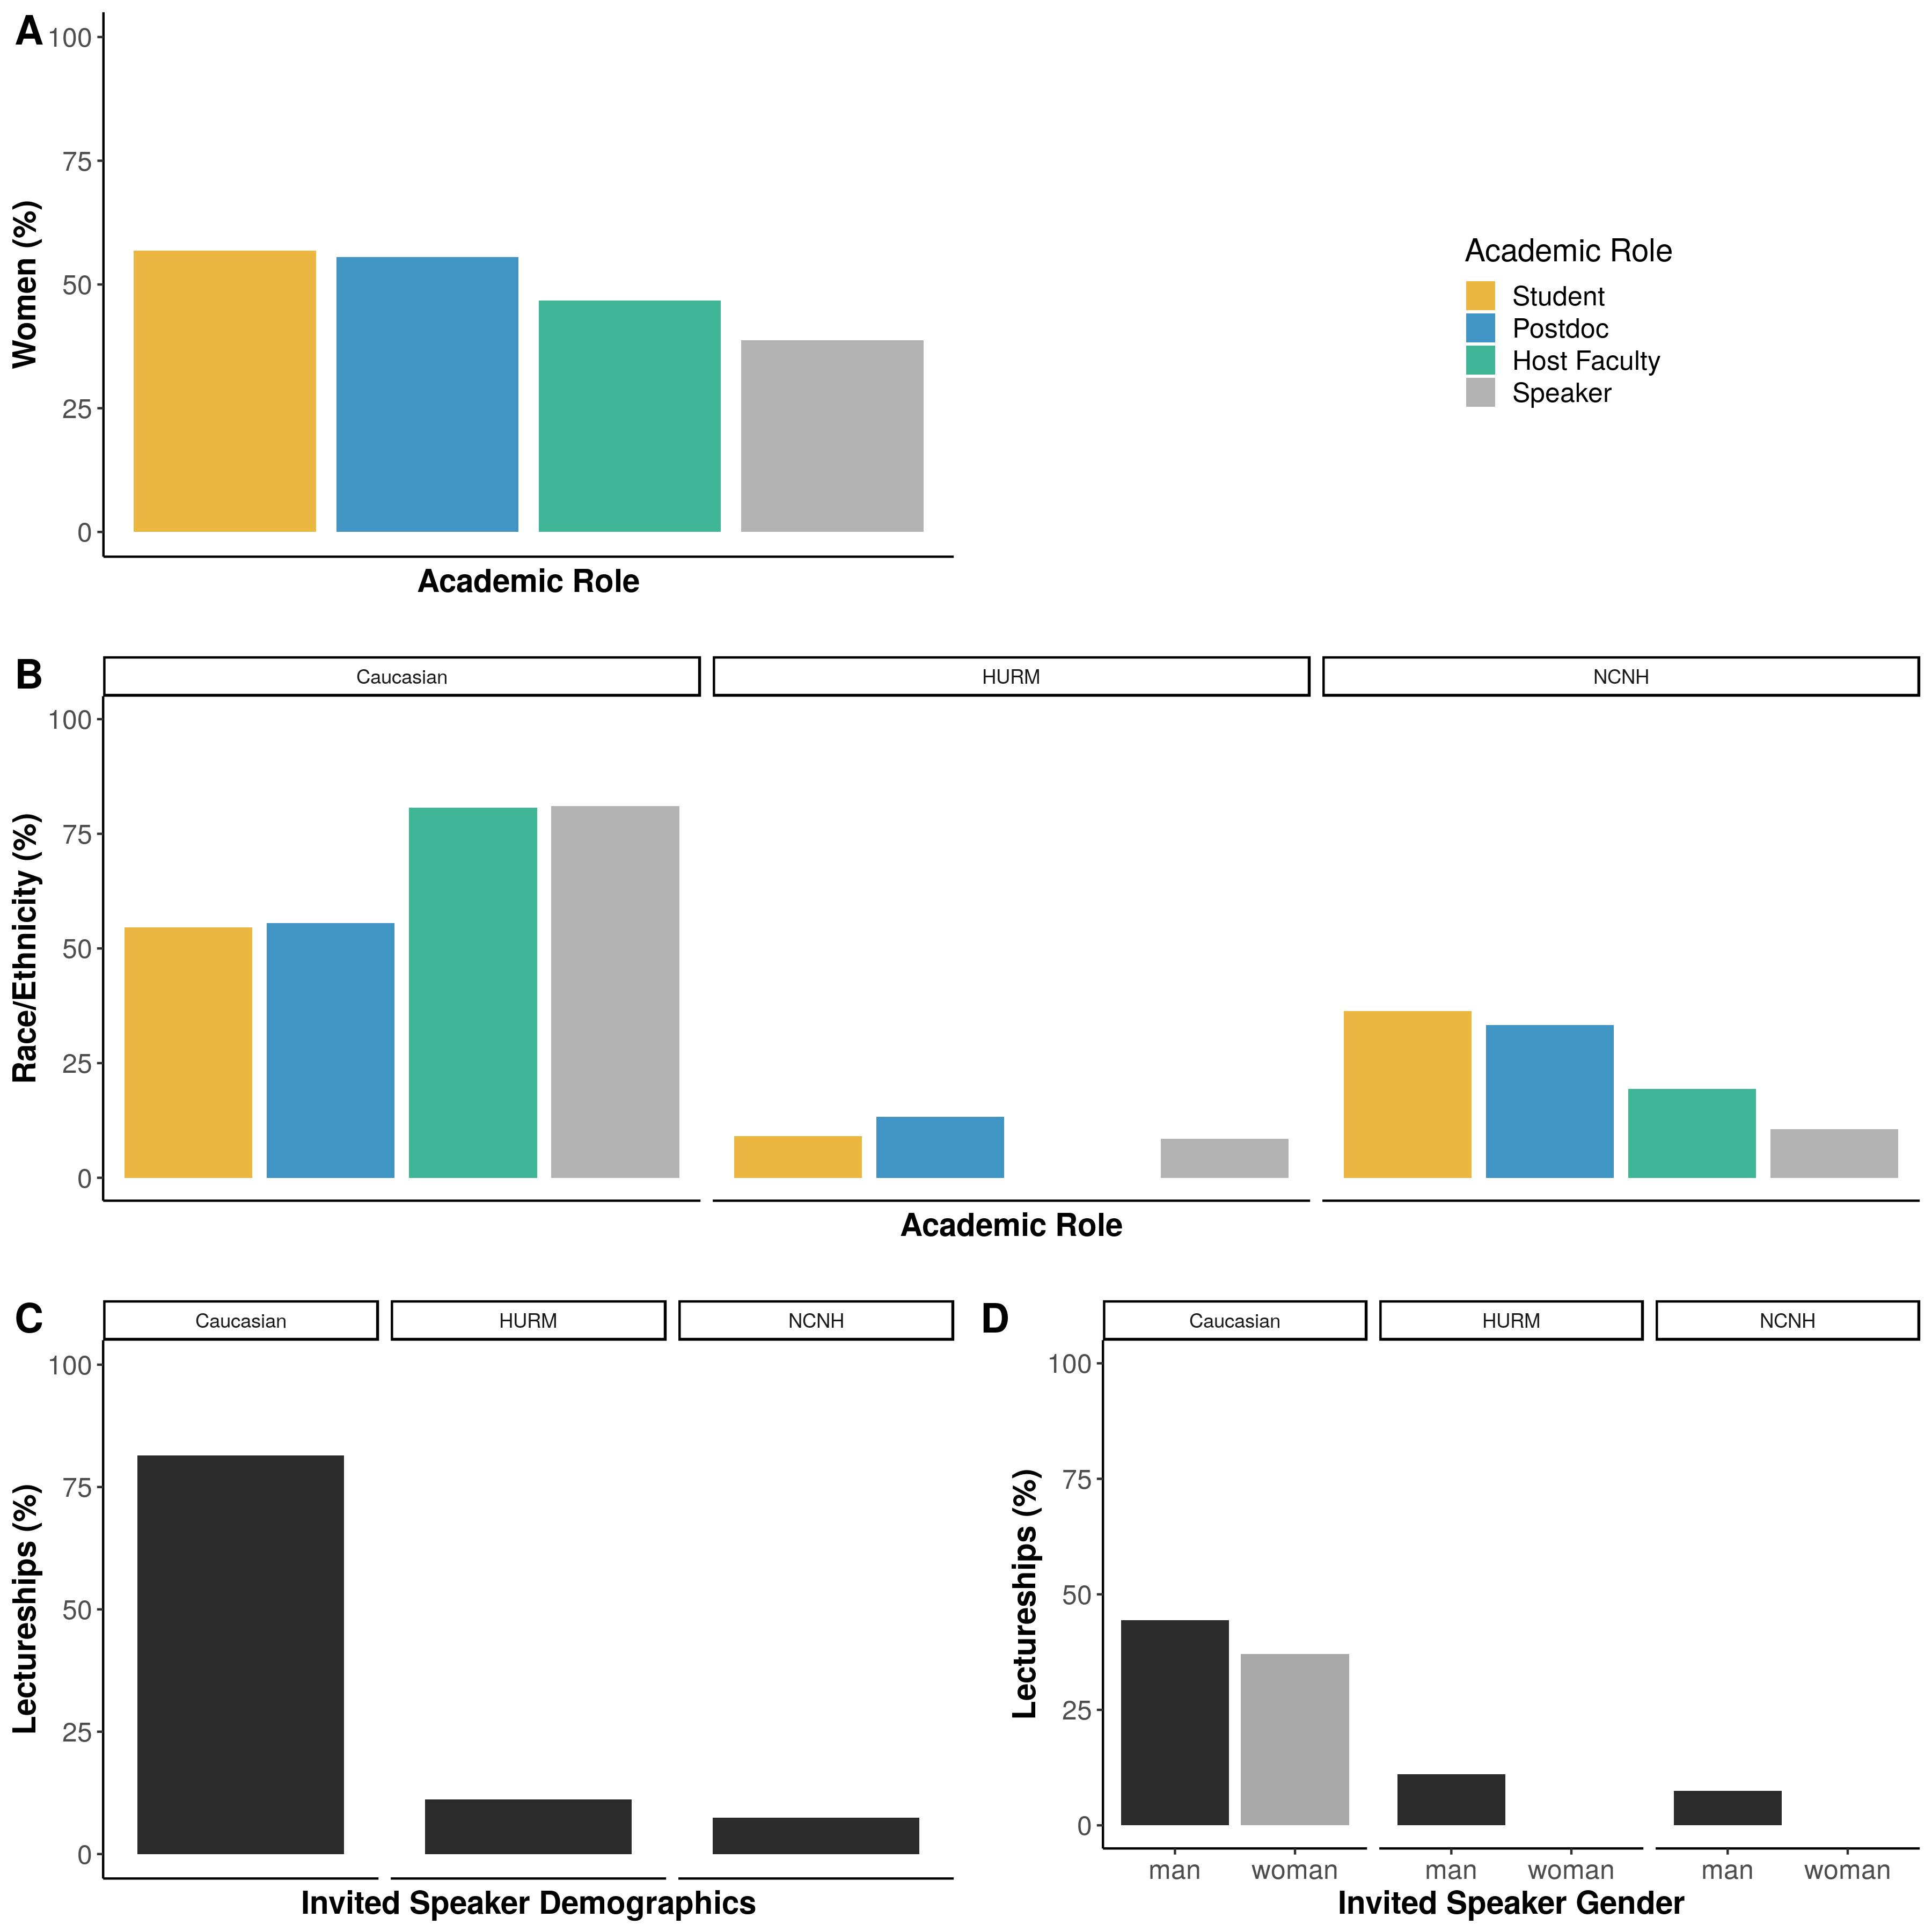
\includegraphics{Figure_1.png}
\caption{Figure 1.}
\end{figure}

Table 1. List of Suggestions \& Resources

\subsection{References}\label{references}

\hypertarget{refs}{}


\end{document}
